\documentclass[a4paper]{article}

\setlength{\parskip}{2mm}
\newcommand{\tab}{~ \qquad}

\usepackage{caratula} 

\usepackage{microtype} % Mejora la tipografía
%\usepackage[utf8]{inputenc} % Para usar caracteres UTF-8

\usepackage{float} % cargar imagenes

\begin{document}

\titulo{Trabajo Práctico}
\subtitulo{Threading}
\fecha{Octubre de 2024}
\materia{Sistemas Operativos}
\grupo{Grupo 25}

\newcommand{\dato}{\textit{Dato}}
\newcommand{\individuo}{\textit{Individuo}}

% Pongan cuantos integrantes quieran
\integrante{Felipe Ignacio Bigiolli}{84/22}{felipebigiolli@gmail.com}
\integrante{Fabrizio Sosa}{1595/21}{fabsosa2727@gmail.com}
\integrante{Matias Neville}{88/22}{nevillematias@gmail.com}

\maketitle

\section{Introducción}

Este trabajo práctico se enfoca en la implementación y sincronización de estructuras de datos concurrentes, específicamente a través del desarrollo de un \texttt{HashMapConcurrente}, una implementación concurrente del tipo abstracto de dato conocido como diccionario. Esta estructura permitirá el acceso seguro por parte de múltiples hilos mediante técnicas de \textit{sincronización}.

Nuestro \texttt{HashMapConcurrente} utiliza hashing abierto, tal que las colisiones son resueltas utilizando listas enlazadas atómicas. El uso de dicha estructura garantiza que, por ejemplo, la inserción de elementos no incurra en race conditions (\textit{condiciones de carrera}).

A lo largo del trabajo práctico, se implementaron mecanismos de sincronización a través del uso de \textit{mutex} y variables o estructuras atómicas, fundamentales para coordinar las operaciones concurrentes. A su vez, se evaluaron estrategias que maximizan la concurrencia sin introducir bloqueos innecesarios, reduciendo así la contención entre los hilos y mejorando el rendimiento de la estructura de datos.


\section{Implementación \texttt{ListaAtomica}}

    La lista atómica es una estructura concurrente diseñada para ser accedida de manera segura por múltiples hilos, garantizando que las operaciones que modifican su estado sean atómicas. Esto significa que las acciones que alteran la estructura interna de la lista, como la inserción de nodos, no pueden ser interrumpidas por otras operaciones concurrentes, con el fin de garantizar la consistencia de los resultados obtenidos por uno o más hilos a la vez. Al utilizar mecanismos de sincronización adecuados, como el uso de semáforos/\textit{mutex}, se asegura que solo un hilo pueda modificar la lista en un momento dado. De este modo, incluso si varios hilos intentan acceder y modificar la lista al mismo tiempo, el resultado final será coherente y equivalente a una ejecución secuencial de las operaciones, protegiendo así a la ejecución general de \textit{race conditions}.

    En cuanto a la operación de inserción (método \texttt{insertar()}), utilizamos un \textit{mutex} para proteger la sección crítica que manipula la cabeza de la lista. Durante la inserción de un nuevo nodo, este se coloca al inicio de la lista, lo que implica modificar tanto el puntero a la cabeza como los enlaces entre nodos. Gracias a utilizar un \textit{mutex}, garantizamos que sólo un hilo tenga acceso exclusivo y pueda realizar estos cambios. Si esta protección no existiera, dos o más hilos podrían intentar modificar la cabeza de la lista simultáneamente, lo que provocaría resultados inconsistentes, como la pérdida de nodos o la corrupción de la estructura interna.


\section{Implementación \texttt{HashMapConcurrente}}

    \subsection{Estructura y funcionamiento de la clase}

    En esta sección, explicaremos el funcionamiento del \texttt{HashMapConcurrente}, haciendo hincapié en los métodos importantes y las decisiones tomadas para garantizar la ausencia de condiciones de carrera y dead-locks. La estructura del \texttt{HashMapConcurrente} está diseñada para manejar múltiples accesos concurrentes de manera eficiente, dividiendo las operaciones en diferentes \textit{buckets} según la primera letra de las claves. Esta división permite que varios hilos operen en paralelo en distintas secciones del diccionario, lo que maximiza el rendimiento y reduce la posibilidad de conflictos entre hilos.

    Recordemos que nuestro \texttt{HashMapConcurrente} resuelve colisiones utilizando listas enlazadas atómicas, de esta manera garantizamos un uso seguro de la concurrencia cuando modificamos cada lista de manera concurrente.

    Se implementaron mecanismos de sincronización para coordinar el acceso a las secciones críticas del código, permitiendo que operaciones como la obtención de claves o valores se realicen sin bloqueos prolongados y evitando la inanición (\textit{starvation}).

    \subsection{Métodos \texttt{incrementar()}, \texttt{claves()} y \texttt{valor()} y su eficiente concurrencia}

    El método \texttt{incrementar()} consiste en, dada una clave, insertar el par $<clave, 1>$ en el bucket correspondiente sí es que no existe, o incrementar el valor de apariciones en 1 si ya existía.

    Nuestra implementación con concurrencia permite que varios hilos realicen dicha modificacion en el \texttt{HashMapConcurrente}, si y sólo si, intentan insertar claves que pertenecen a diferentes \textit{buckets}. Cada \textit{bucket} agrupa las claves según su letra inicial, lo que significa que si dos hilos intentan modificar claves con la misma inicial, alguno de ellos deberá incurrir en algún tipo de espera. El fin de esto es evitar que se produzcan inserciones incorrectas (como la duplicación de una misma clave en lugar de la inserción y posterior actualización de la misma). Para lograrlo, utilizamos mecanismos de exclusión mutua que protegen esta zona critica del código.

    Respecto a la implementación de las funciones \texttt{claves()} y \texttt{valor()}, se tomaron las precauciones necesarias para asegurar que estas también puedan trabajar de manera concurrente con \texttt{incrementar()} sin sufrir condiciones de carrera. Estas dos funciones utilizan una estrategia de sincronización similar. Además, aseguramos que ninguna de estas funciones sufra de inanición.

    La función \texttt{claves()} obtiene todas las claves del \textit{HashMap} concurrente. Para evitar inconsistencias, sincroniza su ejecución de manera que ningún hilo pueda modificar el contenido del \textit{HashMap} (es decir, incrementar los contadores de los \textit{buckets}) mientras se recopilan las claves. Esto garantiza que la lista de claves sea coherente y no se vea afectada por posibles operaciones de escritura concurrentes.

    De forma similar, \texttt{valor()} sincroniza la consulta del valor asociado a una clave específica, permitiendo la lectura solo cuando no hay hilos incrementando el \textit{bucket} correspondiente. Al igual que en \texttt{claves()}, esto asegura que las operaciones de lectura y escritura no interfieran entre sí, manteniendo la coherencia de los datos.

    Estas decisiones de diseño permiten una concurrencia eficiente, evitando bloqueos generales de la estructura de datos o grandes porciones de código, y minimizando la contención entre hilos. Así, logramos que el sistema sea seguro frente a condiciones de carrera, sin comprometer el rendimiento.

    \subsection{Obteniendo promedios de valores}

    \subsubsection{Método \texttt{promedio()} y más problemas de concurrencia a resolver}

    La función \texttt{promedio()} se encarga de calcular la media de los valores almacenados en el hashmap, lo que requiere recorrer linealmente los \textit{buckets} de la tabla. Su ejecución concurrente con la función \texttt{incrementar()} puede dar lugar a problemas de inconsistencia en los datos, ya que \texttt{incrementar()} modifica los valores necesarios para computar el promedio.

    Un escenario que con graves inconsistencias es el siguiente:

    \begin{enumerate}
    \item Partimos de un estado en el que nuestro hashmap no tiene ningun elemento, por lo que la media es 0.

    \item Un hilo comienza a ejecutar \texttt{promedio()} (función que recorre las claves, suma los valores existentes y luego computa el promedio de los mismos).

    \item Supongamos que \texttt{promedio()} ya obtuvo los valores de las letras [a,b,...,y]. Justo antes de obtener el valor de la letra 'z', aparece otro hilo tal que el scheduler le da el procesador y ejecuta las siguientes operaciones: \texttt{incrementar("comillas")}, \texttt{incrementar("zar")}, \texttt{incrementar("comillas")}.

    \item El hilo que ejecutaba \texttt{promedio()} retoma su ejecución, tal que toma el valor de la letra 'z' y computa el promedio. El resultado será $\frac{\sum valores}{\#claves} = \frac{1}{1} = 1$, ya que solo se encontró con la clave-valor $<"zar", 1>$.
    \end{enumerate}

    Esta secuencia de ejecución dio lugar a un resultado inesperado y que no refleja en lo absoluto el verdadero promedio del \textit{hashmap}, pues el verdadero valor es $\frac{2+1}{2} = \frac{3}{2}$

    Para evitar estos problemas de concurrencia, es crucial coordinar las operaciones de lectura y escritura de las estructuras sobre las que trabaja nuestro \textit{hashmap}, de manera que \texttt{promedio()} compute el promedio utilizando los datos del \textit{snapshot} exacto en el que comenzó a ejecutarse, evitando así las interferencias con \texttt{incrementar()}. Esto es resuelto en nuestra implementación de \texttt{promedio()} mediante el uso de los mecanismos de sincronización ya mencionados. Luego, la función \textit{promedio()} recorre cada \textit{bucket} sii no hay ningún hilo incrementando alguna clave. Dado que no hay restricciones sobre tiempos de espera o problemas de inanición, nuestra solución da lugar a que, tanto \texttt{incrementar()} como \texttt{promedio()}, puedan sufrir de inanición si algún hilo realiza una ejecución prolongada y continua de llamadas a alguna de las dos. A modo de resumen, nuestra solución es similar a la del problema de un puente con un único carril bidireccional por el que cruzan autos\footnote{problema y solución visto en clase práctica.\label{fnlabel}}.

    \subsubsection{Implementación de \texttt{promedio\_concurrente()}: una solución más eficiente}

    Si bien la implementación de \texttt{promedio()} garantiza consistencia, existe la posibilidad de optimizar el cálculo en un entorno altamente concurrente. Para mejorar el rendimiento y reducir la espera entre hilos, desarrollamos \texttt{promedio\_concurrente()}: una versión paralela del cálculo de promedio que permite distribuir la carga de trabajo entre varios threads, logrando una mayor eficiencia. Su firma es diferente a la de \texttt{promedio()}, pues esta nueva función recibe un parametro extra que es la cantidad de threads a crear para calcular el promedio.

    La estrategia utilizada para repartir el trabajo de manera óptima es hacer que cada thread se encargue de obtener los valores de un único bucket a la vez. Esto se logra haciendo que los threads trabajen con una variable atómica llamada \texttt{letra\_actual} y otras estructuras de datos lineales. Dicha variable indica la última letra de la cual se obtuvieron los valores. Luego, cada hilo avanza a la siguiente letra en base a la variable atómica, procurando que esta no haya sido ya promediada, ni tampoco sea la de una palabra que esté siendo incrementada. De esta manera, maximizamos la concurrencia, evitando que los hilos bloqueen en \texttt{waits} y siempre estén obteniendo los valores de una letra (o buscando la siguiente letra). Los recursos mencionados que comparten los threads son utilizados dentro de un mutex, ya que es necesario que funcionen de manera atómica para asegurar la correcta sincronización y su lectura y escritura entre los hilos.

    Decidimos que lo más óptimo es que la cantidad de hilos a crear sea el mínimo\{\textit{cant\_threads}, 26\}. Esto porque, sí permitimos más hilos, va a pasar que habrá 26 hilos obteniendo valores de cada uno de los buckets, y los hilos 27°,28°, ..., N° quedaran en un \textit{busy looping} buscando una letra a promediar (lo cual no es posible puesto que sólo hay 26 buckets), tal que provocarían un uso ineficiente de la CPU.

    \subsubsection{Poniendo a prueba a \texttt{promedio\_concurrente()}}

    Para evaluar el rendimiento de \texttt{promedio\_concurrente()}, realizamos una serie de pruebas iterativas para comparar su \textit{performance} respecto a su versión sin concurrencia.
    En el gráfico adjunto, podemos ver cómo varian los tiempos de ejecución de ambas funciones a medida que crecen la cantidad de claves distintas dentro del \texttt{HashMapConcurrente}:

    \begin{figure}[H]
        \centering
        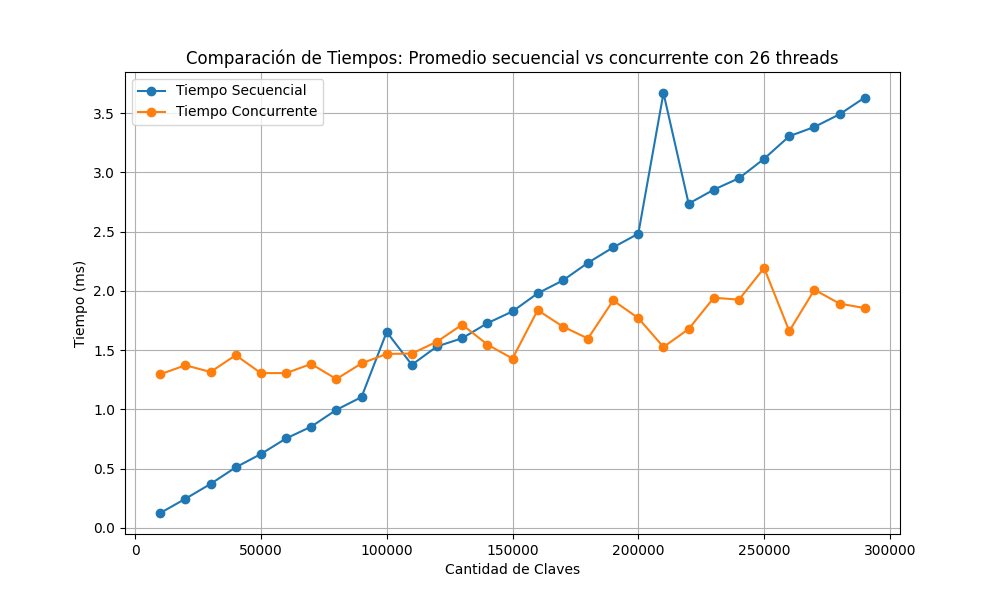
\includegraphics[width=1\textwidth]{codigo/experimentos/comparacion_tiempos.png}
        %\caption{Comparación de tiempos: Promedio secuencial vs promedio concurrente con 26 threads.}
        %\label{fig:comparacion_tiempos}
    \end{figure}

    Podemos apreciar cómo, cuando el diccionario tiene una cantidad de claves en el rango [0,100000], \texttt{promedio()} termina su ejecución en un tiempo menor que su versión concurrente con 26 hilos. Sin embargo, a medida que crece la cantidad de claves totales en el \textit{hashmap},  \texttt{promedio\_concurrente()} logra terminar en un tiempo menor, siendo notablemente superior en rendimiento a la versión no concurrente. Esto la hace mejor para escenarios en los que se trabaje con grandes volúmenes de claves (lo cual continuaremos desarrollando en la conclusión del informe).

    \section{Cargando compras}

    \subsection{Función \texttt{cargarArchivo()}}

    En esta sección, implementamos funciones para la carga automática de compras en nuestro \texttt{HashMapConcurrente}. Para esto, la función \texttt{cargarArchivo()} se encarga de leer el archivo especificado en su parámetro \texttt{filePath} y cargar todas las palabras contenidas en dicho archivo dentro de nuestro diccionario concurrente. A medida que se leen las palabras, se las almacena en el hashMap, incrementando la cuenta correspondiente a la primera letra de cada palabra, utilizando para ello los métodos ya vistos. El proceso es sencillo y no requiere medidas de sincronización adicionales dentro de esta función. Si asumimos que hay 2 o más hilos ejecutando \texttt{cargarArchivo()}, esto no representa un problema aunque estén leyendo el mismo archivo, puesto que sólo lo leen y ejecutan la funcion \texttt{incrementar()}, que, como vimos, está implementada para trabajar en un entorno de concurrencia, sin incurrir en problemas de sincronización como \textit{race conditions}.

    \subsection{Paralelizando la carga de múltiples compras: función \texttt{cargarMultiplesArchivos()}}

    De una forma similar a lo hecho para la función \texttt{promedio()}, implementamos una nueva función que realiza lo mismo que \texttt{cargarArchivo()}, pero utilizando hilos y permitiendo cargar varios archivos a la vez.

    Llamemos N a la cantidad total de hilos, y K a la cantidad total de threads. Enumeremos a los hilos como $t1$, $t2$, ..., $tk$ y a los archivos $a1$, $a2$, ..., $an$.

    La idea de esta función es maximizar concurrencia. Con esto en mente, y para evitar resultados inconsistentes, nuestra solución se basa en que cada thread se encargué de procesar un único archivo en un momento dado. Es decir, si el thread $t1$ está procesando el archivo $a1$, no puede ocurrir que otro thread también lo este haciendo. En otras palabras, se define una "inyectividad" entre los hilos y archivos en todo momento.

    Además, para maximizar la concurrencia, es fundamental que sí un hilo termino de procesar un archivo \( a_J \) (donde \( 1 \leq J \leq N \)), no se quede inactivo. Si \( K < N \), hay más archivos por leer que hilos disponibles, por lo que debemos reasignar el hilo $t1$ (en el contexto de este ejemplo) a otro archivo que no esté siendo procesado por ningún otro hilo.

    En resumen, nuestro enfoque consiste en crear una \textit{pool} de hilos donde cada uno se encarga de un único archivo hasta completarlo. Una vez que un hilo termina de procesar un archivo, debe pasar al siguiente archivo disponible, y así sucesivamente, hasta que no queden más archivos por procesar. Este enfoque busca maximizar la concurrencia y evitar que cualquier hilo se quede esperando a los demás o finalice su trabajo tras procesar un solo archivo, mientras todavía hay tareas pendientes.

    Para implementar esto, utilizamos una variable atómica llamada
    \\ \texttt{indexArchivoAProcesar}, que funciona como un índice para el siguiente archivo a procesar. Esta variable se inicializa en 0 y cada hilo toma el valor de esta variable y lo copia a una variable local. Si el valor era \( J \) (donde \( 1 \leq J \leq N \)), el hilo procesa el archivo $aj$. Luego de copiarlo, incrementa la variable atómica para que el siguiente hilo que la tome procese el archivo  $a_{j+1}$ sii $j+1 < N$.


    \section{Conclusion}
%   a) Ideas sobre puntos de mejora  %
%       - en vez de usar lista enlazada, usar una estructura de datos con mejor perfomance, como un TRIE / PATRICIA (en particular para gestionar strings)  %
%       - permitir más de un hilo dentro de un bucket del hashMap  %
%
%   b) no
%   c)
%

    La estructura de datos \texttt{HashMapConcurrente} presenta una correcta sincronización de sus métodos, tal que pueden ser utilizados en un entorno concurrente. Los métodos claves, como lo son \texttt{incrementar}, \texttt{claves}, y \texttt{promedio} (junto con su versión de múltiples hilos), están protegidos con mecanismos de exclusión mutua para evitar condiciones de carrera, permitiendo operaciones seguras en zonas críticas.

    \subsection{Utilizando el \texttt{HashMapConcurrente} en ventas}

    En un entorno de ventas en línea, como un \textit{e-commerce} que gestiona miles de transacciones por segundo y maneja bases de datos con grandes volúmenes de productos distintos, la eficiencia de las estructuras de datos concurrentes resulta fundamental para mantener el rendimiento del sistema. Como se demuestra en las pruebas de rendimiento de la función \texttt{promedio\_concurrente()} (véase sección 3.3.3), a medida que el número de claves en el \texttt{HashMapConcurrente} supera las 100,000, el rendimiento concurrente se torna notablemente superior al de su versión secuencial. Esta diferencia se acentúa conforme crece el volumen de datos, lo que respalda la implementación del \texttt{HashMapConcurrente} en sistemas de \textit{e-commerce} de gran escala, que podrían trabajar con números con los que la paralelización de ciertas funciones sea más eficiente (como por ejemplo, 150 mil productos distintos), siendo así necesario procesar grandes volúmenes de información en tiempo real de manera óptima, dando como resultado una rápida sensación de \textit{query} para el usuario y una eficiente modificación de las estructuras internas del sistema.

    Sin embargo, un desafío que surge en su implementación es el uso de listas enlazadas concurrentes, como la \texttt{ListaAtomica}, implementada para manejar colisiones dentro de la tabla hash. En un \textit{e-commerce}, es común que múltiples productos compartan la misma clave hash (por ejemplo, productos cuyos nombres comienzan con la misma letra), lo que genera colisiones en los buckets. La búsqueda dentro de estas listas enlazadas tiene un peor caso de $O(n)$, donde $n$ es la cantidad de productos que comparten la misma letra o prefijo.

    Para mejorar la eficiencia, se puede utilizar otra estructura de datos para gestionar las colisiones de cada bucket. Por ejemplo, se podria utilizar un trie-PATRICIA
    \footnote{Brass, P. (2008). \textit{Advanced Data Structures}. Chapter 8.1: Tries and Compressed Tries.\label{fnlabel}}.
    Esta estructura ofrece un mejor rendimiento en la búsqueda, reduciendo el tiempo de acceso en casos de colisiones y mejorando así el rendimiento global del sistema de ventas, particularmente bajo una carga concurrente elevada.

    Siguiendo esta linea, consideramos que otro punto de mejora sería permitir que varios hilos tengan acceso a un mismo bucket.

    Consideramos que nuestra solución resulta práctica para un \textit{e-commerce} que maneje una gran cantidad de productos y ventas, pues en caso contrario esta solución con concurrencia no es necesaria. En nuestra implementación, se emplean múltiples variables y estructuras diseñadas para sincronizar procesos concurrentes, lo cual introduce un alto grado de complejidad a la estructura. Esta complejidad sólo se justifica cuando hay una carga significativa de trabajo, como un gran número de productos o transacciones simultáneas. Por lo tanto, si la tienda tiene pocos productos, el esfuerzo de implementar mecanismos de sincronización sería innecesario, ya que el esfuerzo que esto implica no se traduciría en una mejora tangible del rendimiento.

    \subsection{Añadiendo \textit{features} a la estructura}

    Dada la implementación presentada de \texttt{HashMapConcurrente}, resulta simple añadir funcionalidades nuevas re utilizando estrategias de sincronización como las de \texttt{promedio\_concurrente}. Luego, podemos obtener otras métricas, como la mediana.

    Obtener la mediana de un conjunto de datos consiste en ordenar dicho conjunto de menor a mayor y, en función de $n$ (siendo $n$ la cantidad de elementos de la muestra), obtener el valor que se encuentra justo en el medio; se la expresa como $\frac{x_{n/2} + x_{(n/2)+1}}{2}$  si n es par  o  $\frac{x_{n+1/2}}{2}$ si n es impar.

    Luego, debemos obtener los datos y ordenarlos de manera ascendente. El problema resulta así muy similar al calculo del promedio concurrente: obtenemos los datos utilizando hilos de manera paralela y computamos la respuesta.

    Se puede plantear una solucion en la que cada thread recorra un bucket e inserte los elementos en un heap (lo cual supone una complejidad de $O(n\ log\ n)$). Finalmente, calculamos la mediana extrayendo los primeros $n/2$ elementos (y leyendo el elemento $n/2 + 1$). La complejidad total es $O(n\ log\ n)$, pues la complejidad cada extracción del heap es $O(log\ n))$

\end{document}

